
\section{Server applikation}

Sammenhængen mellem Webapplikationen og Web-serveren kan beskrives som en MVC-løsning, hvor Webapplikationen fungere som view, og Web-serveren som Model-Controller. Dog er dette en grov simplificering af interaktionen, men beskriver forholdet mellem de forskellige parter. Webapplikationen skal kommunikere med Web-serveren, som ikke kun er en enkelt server, men en samling af dem som arbejder parallelt, kaldet et cluster. Denne cluster fungerer som en web-server. Dette er valgt for at give muligheden for at arbejde parallelt på de forskellige services, samt at fremstille serveren efter Domæne-Drevet-Design (DDD) \cite[DDD]{converge-terms}, hvilket grupperer funktionalitet efter relevans for forretningsdomænet: krav og kontekst \cite{documentation-kravspec}.

Web-serveren har en primær funktion: At behandle anmodninger med passende forretningslogik. Adgangen til denne forretningslogik foregår igennem forskellige adresser på Web-serveren. Disse adresser udgår på den udstillede Web-server API. Det skal siges at Web-serveren og Converge-Cluster er forskellige men benyttes til samme formål, Det vil sige hvor Web-serveren beskriver selve ideen fra et overbliks perspektiv, og Converge-Cluster for det egentlige produkt.

Derudover vil Web-serveren ved behandling af anmodninger gemme resultater i et persitteringslag \cite[Permitteringslag]{converge-terms}, enten som filer eller rækker i en database. Denne information skal kunne hentes til den funktion der har brug for det, og som har adgang. De forskellige services (selvstændige applikationer) i Web-serveren,  består af $n$ lag: Et samlingslag, Et præsentationslag (API), et forretningslag (forretningslogik), og et dataadgangslag. Disse fire lag placeres i en teknologisk sammenhæng, hvor ASP.NET Core platformen er valgt. Denne platform har programmerbar routing, der samler alle kald til de individuelle services.

Resten af afsnittet indeholder uddrag fra dokumentation \cite{software-architecture}.

\begin{figure}[H]
  \begin{small}
    \begin{center}
      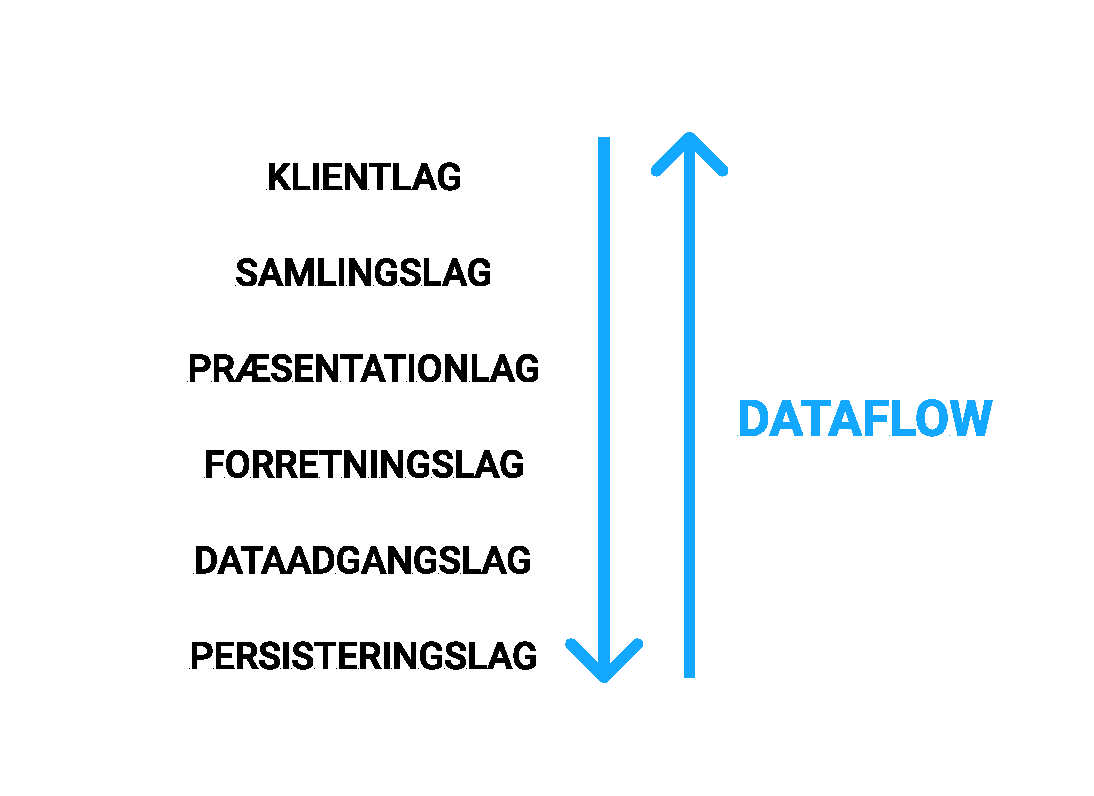
\includegraphics[width=0.55\textwidth]{Billeder/N-lag.pdf}
    \end{center}
    \caption{N-lags struktur}
    \label{fig:n-layer}
  \end{small}
\end{figure}

\textbf{Klientlag} anvender de underliggende lag, til at præsenterer og interagerer med brugeren. Klientlaget, vil være enten en tredjepart, eller Klientapplikationen.

\textbf{Samlingslaget} samler de underliggende applikationer under én udgang, dette gør det muligt for Web-applikationen at nemt kunne skifte mellem de forskellige services og endpoints. Samlingslaget må ikke indeholde forretningslogik, og skal bare beskytte de bagvedliggende services.

\textbf{Præsentationslaget} præsenterer et JSON API til omverdenen. Dette API forventes at modtage JSON \cite[JSON]{converge-terms} indpakket data ved anmodninger, og ingen data ved forespørgsler. Præsentationslaget er tyndt og indeholder kun lige nok data til at verificere indholdet, samt at verificere klienters anmodningsrettigheder. Det forventes at hvis en anmodning er valideret, vil den blive sendt videre til forretningslaget, hvilket kan håndtere dette. Alt i alt vil det sige at data kan modtages og returneres i dette lag, men kun det overfladiske er valideret, resten er bestemt i forretningslaget.

\textbf{Forretningslaget} indeholder services, der agerer på klienters forespørgsler i systemets domæne. Her bliver forespørgsler håndteret baseret på forretningslogik. Dette kan f.eks. være kommunikation til andre services, for at få deres ressourcer eller videresende begivenheder til interesserede parter.

\textbf{Dataadgangslaget} er bygget op omkring 2 forskellige services; enten en http-klient eller en databaseadgangsklient. Til en http-klient er der brugt et fælles bibliotek der kan tilgå systemets ressourcer, dette gør at to forskellige services kan tale sammen, selvom man skriver C\# kode. Til en databaseadgangsklient er der brugt repositories - ved et repository beskriver man hvordan databasen skal tilgås. Repositories udgiver en grænseflade som er implementeret med den klient kode der skal til for at kommunikere med database. I dette tilfælde er MongoDBClient brugt, pga. databasetypen som er MongoDB.

\textbf{Persisteringslag} Dette lag håndeterer persisteringen af data. Dette kan gøres med en hvilken som helst database, dog skal det understøtte MongoDBClient.

Server applikationen skal agere som en fælles front, men have forskellige  bagvedliggende komponenter. Nogle som præsenterer et nemt anvendelige måde at bruge grænseflade, og andre lidt mere komplekse som bruges inde i selve systemet. I dette tilfælde kan det f.eks. være til Users Service, hvilket er en af byggestenene for systemet, det beskriver noget om brugeren og indeholder et id som bruges i næsten alle andre services. Users service bliver f.eks. brugt af authentication-service som skal udstede et API til registrering og login - dvs. at Users service primært er længere nede i hierarkiet end authentication-service.